\documentclass[11pt]{article}
%\documentclass[aps,preprint,superscriptaddress,11pt]{revtex4-1}
%\renewcommand{\familydefault}{\sfdefault}
%\usepackage{arial}
%\usepackage{arial}
%\renewcommand{\familydefault}{\sfdefault}

\renewcommand{\rmdefault}{phv} % Arial
\renewcommand{\sfdefault}{phv} % Arial
\usepackage[pdftex]{graphicx}
\usepackage{scrextend}
\usepackage{hyperref}

\usepackage{enumitem}
\setlist[1]{itemsep=-3pt,topsep=-3pt}

% Include figure files
\usepackage{bm}
\usepackage{graphicx}
\usepackage{subfig}
\usepackage{lscape}
\usepackage{empheq}
\usepackage[usenames,dvipsnames]{color}
%\usepackage[framemethod=tikz]{mdframed}                                                                                                     
\usepackage{amsfonts}
\usepackage{amsmath}
\usepackage{amsthm}
\usepackage{multirow}
\usepackage{bbold}
\usepackage[varg]{txfonts}
\usepackage{feynmp}
\DeclareGraphicsRule{*}{mps}{*}{}
\definecolor{eqcolor}{gray}{.9}
\usepackage{todonotes}

%\usepackage[justification=justified]{caption}
\usepackage{dcolumn}% Align table columns on decimal point
\usepackage{bm}% bold math
\usepackage{color}
\usepackage{subfig}
\usepackage{xspace}
\usepackage{lineno}
\usepackage{hyperref}% add hypertext capabilities
\usepackage{natbib}
\usepackage{ulem}
\usepackage{multicol}
\usepackage{eurosym}
\usepackage{enumitem}
\usepackage{setspace}
%\usepackage[mathlines]{lineno}% Enable numbering of text and display math
\usepackage[utf8]{inputenc}

%\RequirePackage{lineno}
%\linenumbers\relax % Commence numbering lines
%\input symbols
\setlength
\linenumbersep{0.1cm}
%\linenumbers\relax % Commence numbering lines
%\usepackage[showframe,%Uncomment any one of the following lines to test 
%%scale=0.7, marginratio={1:1, 2:3}, ignoreall,% default settings
%%text={7in,10in},centering,
%%margin=1.5in,
%%total={6.5in,8.75in}, top=1.2in, left=0.9in, includefoot,
%%height=10in,a5paper,hmargin={3cm,0.8in},
%]{geometry}

%% page setup
\setlength{\hoffset}{-14mm}  
\setlength{\voffset}{-10mm}
\setlength{\textwidth}{175mm}
\setlength{\oddsidemargin}{12mm}
%\setlength{\textheight}{247mm}
\setlength{\textheight}{237mm}
\setlength{\topmargin}{-25mm}
\setlength{\headheight}{20mm}
\setlength{\headsep}{5mm}
\setlength{\footskip}{13mm}
\newlength{\capindent}
\setlength{\capindent}{1.0cm}
\newlength{\capwidth}
\setlength{\capwidth}{\textwidth}
\addtolength{\capwidth}{-2\capindent}

%% colours (see http://en.wikibooks.org/wiki/LaTeX/Colors) and fonts
\newcommand\introTitleColor{\color{Cerulean}}
\definecolor{darkmidnightblue}{rgb}{0.0, 0.2, 0.4}
%\newcommand\hkTitleColor{\color{BlueViolet}}
\newcommand\hkTitleColor{\color{darkmidnightblue}}
\definecolor{americanrose}{rgb}{1.0, 0.01, 0.24}
\newcommand\hkCommentColor{\color{americanrose}}
\definecolor{mediumred-violet}{rgb}{0.73, 0.2, 0.52}
\renewcommand*{\familydefault}{\sfdefault}
\newcommand\introNewParagraph{
  \smallskip
  \noindent
}
%%%
\newcommand{\FHC}{\ensuremath{\nu}-mode\xspace}
\newcommand{\RHC}{\ensuremath{\overline{\nu}}-mode\xspace}

\renewcommand{\baselinestretch}{1.}\normalsize

\begin{document}

\pagenumbering{roman}
\setcounter{page}{1}

%\newcommand{\thetacerenkov}{$\theta_{\mathrm{Cerenkov}}$}

%\graphicspath{{img/}}
%
\begin{flushright}
%\today\\
September 5, 2016\\
\end{flushright}
\vspace{5ex}
\centerline{\introTitleColor\Huge \bf Statement of Interest}
\centerline{\introTitleColor\Huge \bf for the Hyper-Kamiokande Experiment}
%
\vspace{5ex}
\bigskip

%\begin{center}
%{\introTitleColor\Large\bf HyperK}\\
P.\ Beltrame, 
G.A.\ Cowan, 
M.\ Needham, 
S.\ Playfer, 
G.\ Sidiropoulos 
(University of Edinburgh); 
P.\ Dunne,
P.\ Jonsson,
P.\ Litchfield,
Y.\ Uchida, 
M.O.\ Wascko 
(Imperial College London); 
T.\ Dealtry, 
A.\ Finch, 
L.\ Kormos, 
H.\ O'Keeffe (Lancaster University);
C.\ Andreopoulos, 
N.\ McCauley, 
D.\ Payne, 
J.\ Rose (University of Liverpool); 
G.\ Barr, 
D.\ Wark 
(University of Oxford); 
F.\ Di Lodovico, 
K.\ Hayrapetyan,
T.\ Katori,
A.\ Owen, 
R.\ Sacco, 
S.\ Short, 
R.\ Terri, 
J.\ Wilson,
B.\ Richards 
 (Queen Mary University of London); 
T.\ Berry, 
A.\ Kaboth,
J.\ Monroe 
(Royal Holloway University of London);
S.\ Cartwright, 
M.\ Malek, 
J.\ Perkin, 
L.\ Thompson (University of Sheffield); 
C.\ Densham, 
M.\ Fitton, 
T.\ Davenne, 
T.\ Nicholls, 
T.\ Stewart, 
M.\ Thorpe, 
A.\ Weber  
(STFC/RAL); 
G.\ Barker, 
S.\ Boyd, 
D. Hadley (University of Warwick).
%\end{center}

\vspace{5ex}
%
%
%
%\thispagestyle{empty}
\hspace{0.5cm}
\begin{figure}[htb]
\begin{center}
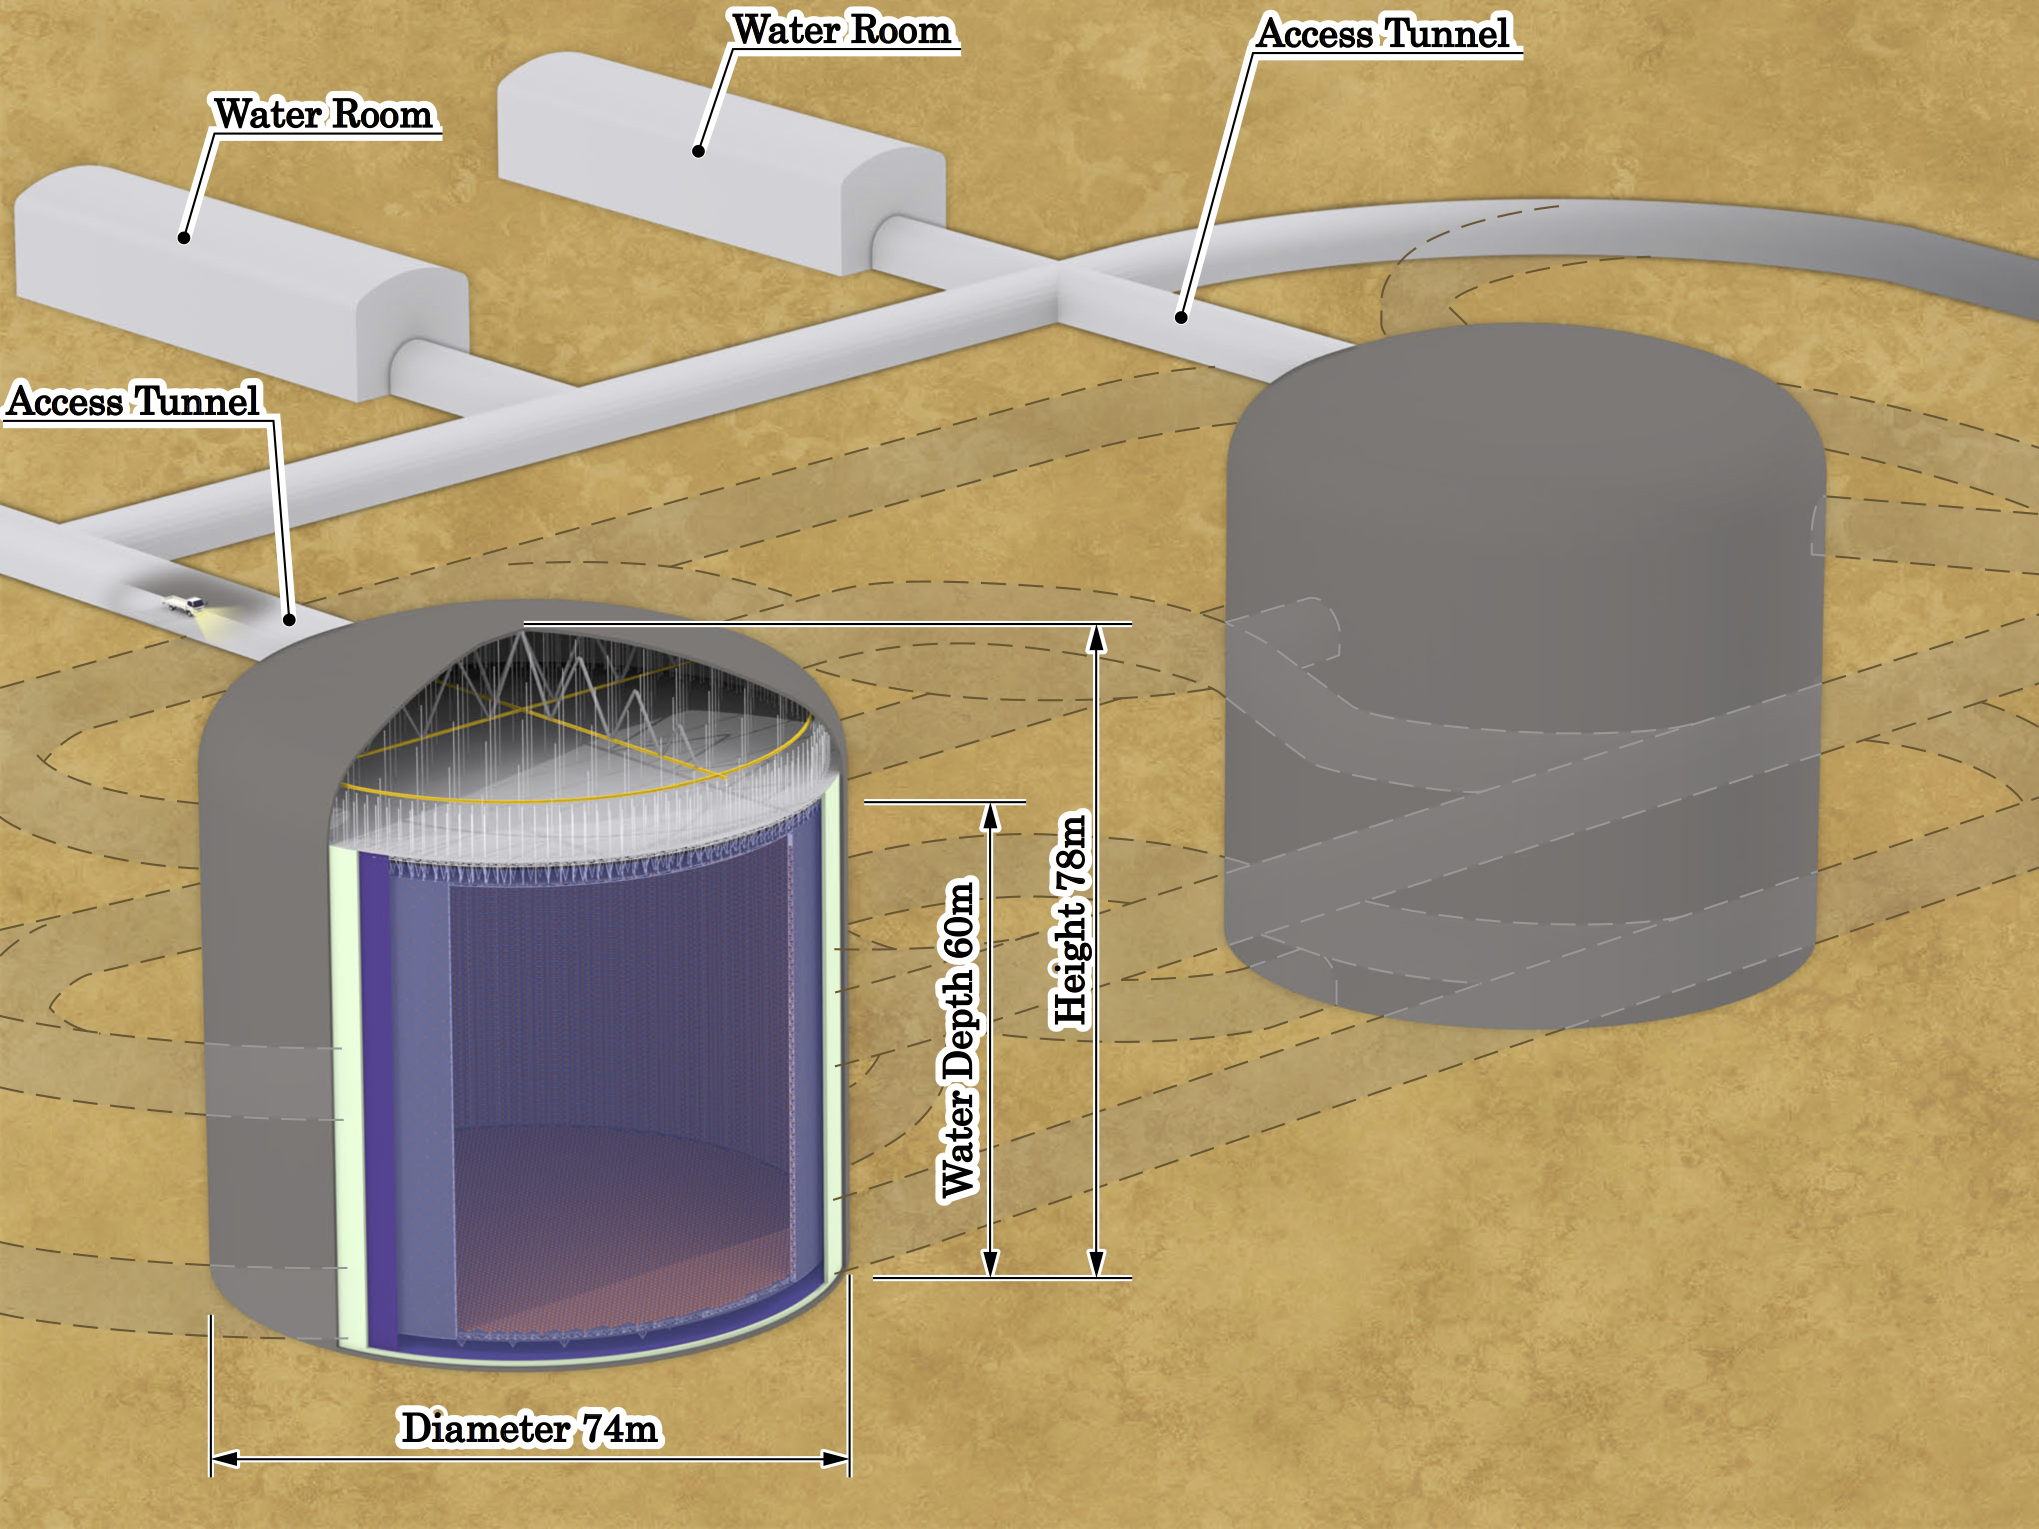
\includegraphics[scale=0.25]{figs/hyperk.png}
%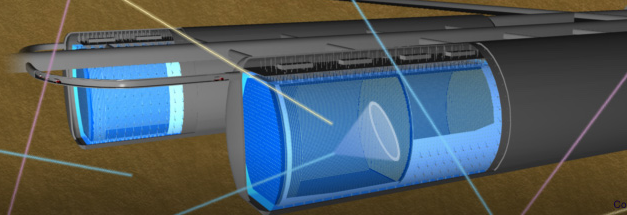
\includegraphics[scale=.7]{figs/hyperk-main.png}
\end{center}
%%\vspace{-3.5cm}
\end{figure}

\hspace{0.1cm}
\vspace{1ex}

\begin{figure}[htb]
\begin{center}

\includegraphics[scale=.4]{figs/edinburgh.jpg}
\vspace{.2cm}

\includegraphics[scale=0.4]{figs/ic.jpg}
\vspace{.2cm}

\includegraphics[scale=.4]{figs/lancaster.png}
\vspace{.2cm}

\includegraphics[scale=.3]{figs/liverpool.jpg}
\vspace{.2cm}

\includegraphics[scale=0.15]{figs/oxford.png}
\vspace{.2cm}\\

\includegraphics[scale=.4]{figs/qmul.jpg}
\vspace{.2cm}

\includegraphics[scale=.2]{figs/rhul.jpg}
\vspace{.2cm}

\includegraphics[scale=0.3]{figs/sheffield.png}
\hspace{.2cm}

\includegraphics[scale=0.5]{figs/RAL.png}
\vspace{.2cm}

\includegraphics[scale=.2]{figs/warwick.jpg}
\end{center}
%%\vspace{-3.5cm}
\end{figure}
\newpage

\makeatletter
\let\toc@pre\relax
\let\toc@post\relax
\makeatother
%\tableofcontents

\newpage

Hyper-Kamiokande is the flagship experiment in Japan. It is the latest
in the generation of highly successful Kamiokande experiments with the
T2K, Super-Kamiokande and Kamiokande experiments (awarded a
Breakthrough prize, and two Nobel prizes respectively) as its
predecessors.

The experiment will be developed by an international collaboration
that will inherit the expertise and experience to provide a
world-leading experiment capable of addressing the biggest unsolved
questions in physics through an exciting multi-decade physics
programme that will start in the middle of the next decade.

The Hyper-Kamiokande detector will be hosted in the Tochibora mine,
about 295\,km away from the J-PARC proton accelerator research complex
in Tokai, Japan. A new cavern will be excavated and necessary
infrastructure will be built. The detector will be the largest
underground water Cherenkov detector in the world and will be
instrumented with new technology photosensors, faster and with higher
quantum efficiency than the ones in Super-Kamiokande. Pressure tests
demonstrate that they will be able to withstand the pressure exerted
by a massive tank.

The currently existing accelerator serving the T2K experiment will be
steadily upgraded to reach a 1.3\,MW beam before the start of the
experiment. Enhancements to the existing array of near detectors will
provide a precision tool for investigating the CP violating nature of
the neutrino. The enhancements will consist of upgrades and new
detectors at a distance ranging from 280\,m to 1-2\,km from the
neutrino target.

A recent new proposal includes a second detector in Korea that will be
able to further augment the physics of the first detector in Japan.

The science that will be done will shape the future theoretical
framework and generations of experiments. The experiment will be
sensitive to beam and atmospheric neutrinos. It will be able to
measure with the highest precision the leptonic CP violation that
could explain the baryon asymmetry in the Universe. A precise
measurement of the other oscillation parameters will be performed,
including the determination of the $\theta_{23}$ octant and mass
hierarchy.  The unprecedented precision and sensitivity of the
experiment will enable a detailed study of the nature of the neutrino
to be made allowing deviations from the three flavour neutrino mixing
to be studied and enable new phenomena searches to be made.

The experiment will also have excellent sensitivity and precision for
proton decay studies, providing a significant improvement over
existing or planned experiments. strong astrophysical programme will
be carried out at the experiment that will also allow to measure
precisely solar neutrino oscillation. A program of other main physics
searches are planned such as indirect dark matter.

In summary, a new experiment, based on the experience and facilities
of the already existing Super-Kamiokande and long baseline neutrino
experiment T2K, is being developed by the international physics
community to provide a wide and groundbreaking multi-decade physics
programme from the middle of the next decade.  The beam upgrade for
the Hyper-Kamiokande experiment is the highest priority for the KEK
lab and it is already approved. The PMT specifications should be ready
by the end of 2017. Already preaparation for their mass production has
started with the creation of a new Hamamatsu mass production 
factory. Finally, a Memorandum of Understanding for the cooperation in
supporting Hyper-Kamiokande has been signed by the KEK/IPNS and
University of Tokyo/ICRR.

The international community is composed of 13 Countries, the UK is the
largest in size outside of Japan.  International contributions include
the beam, near/intermediate detectors, half of the photodetection system
for Hyper-Kamiokande as well as the DAQ and electronics. The second
tank in Korea contribution is currently being discussed.
The UK contributions span the complete experiment configuration from
the beam through to the near and intermediate detectors and finally
the far detector(s). The UK contributions will also include the
computing infrastructure and tools necessary to successfully deliver
world's best measurements.\\

{\bf Beam:} The UK have made key contributions to the existing T2K
facility, including the beam window, baffle collimator and target
system for operation at up to 0.75\,MW. As beam powers increase to the
MW level, the beam window and target in particular are expected to
become limiting technologies.  We continue to keep our leadership in
the beam for the update up to 1.3\,MW. We will focus our efforts on
upgrading the target and beam window to operate reliably at the
1.3\,MW beam power based on an evolution of the current monolithic
target, potentially a good solution for the upgraded beam
conditions.\\

{\bf Near detector:} The T2K near detector is fundamental to
understanding the beam before oscillation, and constrains the expected
spectrum at the far detector through the direct measurement of the
beam flux and cross sections.  We aim to add a new detector, the High
Pressure TPC.  Gas detectors allow detection and reconstruction of
very low momentum particles, which significantly improves the ability
of neutrino experiments to distinguish between neutrino interaction
models and test them against data in regions of phase space that were
not accessible to previous experiments.\\

{\bf Intermediate detector:} As demonstrated by the T2K near detector,
it is crucial to use the same target material, water, as at the far
detector. This is necessary for reducing the systematic errors on the
measurements which is essential for CP violation measurements.
Furthermore, a location around 1-2\,km will minimize the beam
errors. We will work on a water Cherenkov at 1-2\,km, and we envisage
using gadolinium-doped water to identify neutrino and antineutrino
interactions with neutrons in the final state.\\

{\bf Far detector:} Three main contributions are planned for the far
detector: DAQ, calibration and outer detector (OD). The DAQ and
calibration systems will also be adapted to the intemediate detector
which will use the same technology as the far detector.\\

{\underline{DAQ}:} The UK is responsible for all the T2K near detector
DAQ, and aims to include responsibilities for the DAQ for the
intermediate and far detectors. A robust DAQ system capable of
achieving the maximum physics reach in all areas is required. A
framework DAQ has been developed and will need to be adapted to the
final chosen PMTs and electronics.\\

{\underline{Calibration}:} We have a strong experience in the
calibration in SNO and SNO+ on which we base our contribution to the
calibration. To meet the Hyper-Kamiokande physics goals, it is
necessary to reduce both the errors in photodetector calibration and
the uncertainties in the reconstruction efficiency of the neutrino
events. We have a total of three calibrations that we are developing
and also possibly test in Super-Kamiokande. The calibration methods
will also be applied to the intermediate detector.\\

{\underline{Outer Detector}:} As demonstrated in Super-K, the OD is
crucial to provide a background reduction, tagging the external
backgrounds. An original design using smaller PMTs than in Super-K
allows to engage a UK company for the development and future
production.\\

{\bf Computing \& Software:} The UK is responsible for the software
release management and data distribution, that is supported by the
GridPP in the UK. We are also responsible for the triggering and low
energy simulation for the Hyper-K simulation package.\\

{\bf Physics:} The UK is leading the oscillation analysis in T2K, and
adapting those techniques, is now providing the sensitivities
estimates for Hyper-Kamiokande.\\

Discussions for the second tank in Korea are preliminary, but we may
provide the DAQ and calibration also for the Korean detector.

The UK have leadership roles in all the areas we work demonstrating
the indispensible contribution the UK is making to the
experiment. Strong connections with the UK industries are being
developed.

Finally, the current work will be able to provide training in
technical skills for STEM, leading to a skilled workforce with an
improved understanding of technology and its relevance for science,
leading to an increased revenue generation for the UK, and a more
technically literate society. We address several projects for students and
a variety of occasions to communicate the physics to the wider public.


%\begin{itemize}
%
%    \item Physics Motivation (1 pages)
%    \item The Hyper-Kamiokande overview (2 pages)
%    \begin{itemize}
%        \item J-PARC facility, beam-line, and near detector system
%        \item Water Cherenkov detector
%        \item International organizaton
%    \end{itemize}
%
%    \item Hyper-K Physics cases (5 pages)
%    \begin{itemize}
%        \item Accelerator-based neutrino oscillations and $CP$ violation
%        \item Neutrino oscillation studies by atmospheric (and solar neutrinos)
%        \item Astrophysical neutrinos from Supernova, Sun, and other sources
%        \item GUT test by nucleon decays
%    \end{itemize}
%
%\end{itemize}

%Hyper-Kamiokande will be a next generation underground water Cherenkov
%detector with a total (fiducial) mass of 0.99 (0.56) million metric
%tons, approximately 20 (25) times larger than that of
%Super-Kamiokande.  

%One of the great strengths of the Hyper-K program
%is its wide ranging physics program.  For searches from astrophysical
%neutrinos from sources as diverse as dark matter and supernova, to
%tests of the stability of matter, along with a comprehensive study of
%neutrino oscillations and CP violation using both atmospheric and
%accelerated based neutrinos, Hyper-K offers a broad and deep program
%of physics.  These topics are introduced in this section, and the
%details of Hyper-K's sensitivity to the various items are explored in
%depth in~\ref{section:physics}.  As an overview, a list of physics
%topics along with the physics sensitivity or potential of each in the
%Hyper-K program is summarized in Table~\ref{tab:intro:phys}.
%
%\begin{table}[hbtp]
%  \caption{Physics targets and expected sensitivities of the Hyper-Kamiokande experiment.} 	
%  \label{tab:intro:phys}
%  \begin{center}
%    \begin{tabular}{lll} \hline \hline
%      Physics Target & Sensitivity & Conditions \\
%      \hline \hline
%      Neutrino study w/ J-PARC $\nu$~~ && 7.5\,MW $\times$ $10^7$ sec\\
%      $-$ $CP$ phase precision & $<19^\circ$ & @ $\sin^22\theta_{13}=0.1$, mass hierarchy known \\
%      % && mass hierarchy (MH) is known \\
%      $-$ $CPV$ discovery coverage & 76\% (3\,$\sigma$), 58\% ($5\,\sigma$) & @ $\sin^22\theta_{13}=0.1$, mass hierarchy known \\
%      % & 58\% ($5\sigma$) \\
%      % & 74\% (63\%) & @ $s^22\theta_{13}=0.03$, MH known(unknown) \\
%      % & 66\% (59\%) & @ $s^22\theta_{13}=0.01$, MH known(unknown) \\
%      $-$ $\sin^2\theta_{23}$ & $\pm 0.015$ & 1$\sigma$ @ $\sin^2\theta_{23}=0.5$ \\
%      \hline
%      Atmospheric neutrino study && 10 years observation\\
%      $-$ MH determination & $> 3.8\,\sigma$ CL & @ $\sin^2\theta_{23}>0.4$ \\
%      $-$ $\theta_{23}$ octant determination & $> 3\,\sigma$ CL & @  $|\theta_{23} - 45^{\circ}| > 8^{\circ}$ \\\hline
%      \hline
%      Atmospheric and Beam Combination && 10 years observation\\
%      $-$ MH determination & $> 6.9\,\sigma$ CL & @ $\sin^2\theta_{23}>0.4$ \\
%      $-$ $\theta_{23}$ octant determination & $> 3\,\sigma$ CL & @  $|\theta_{23} - 45^{\circ}| > 3^{\circ}$ \\\hline
%      %
%     Nucleon Decay Searches && 5.6 Mton$\cdot$year exposure \\
%      $-$ $p\rightarrow e^+ + \pi^0$ & $9.3 \times 10^{34}$ yrs (90\% CL UL) &\\
%                     & $4.3 \times 10^{34}$ yrs ($3\,\sigma$ discovery) &\\
%      $-$ $p\rightarrow \bar{\nu} + K^+$ & $2.7 \times 10^{34}$ yrs (90\% CL UL) &\\
%                     & $0.9 \times 10^{34}$ yrs ($3\,\sigma$ discovery) &\\ 
%      \hline
%      Astrophysical neutrino sources && \\
%      $-$ $^8$B $\nu$ from Sun & 200 $\nu$'s / day & 7.0\,MeV threshold (total
%                                                     energy) w/ osc.\\
%                                                     % $-$ $^8$B $\nu$ day/night accuracy & $<1\%$ & 5 years, only stat. w/ SK-I BG $\times 20$\\ \hline
%                                                     % Astrophysical objects &&\\
%      $-$ Supernova burst $\nu$ & 170,000$\sim$260,000 $\nu$'s & @ Galactic center (10 kpc)\\ 
%                     & 30$\sim$50 $\nu$'s & @ M31 (Andromeda galaxy) \\ 
%      $-$ Supernova relic $\nu$ & 830 $\nu$'s / 10 years & \\
%      $-$ WIMP annihilation at Sun & & 5 years observation\\
%      ~~($\sigma_{SD}$: WIMP-proton spin & $\sigma_{SD}=10^{-39}$cm$^2$ & @ $M_{\rm WIMP}=10$\,GeV, $\chi\chi\rightarrow b\bar b$ dominant\\
%      ~~~~dependent cross section)& $\sigma_{SD}=10^{-40}$cm$^2$ & @ $M_{\rm WIMP}=100$\,GeV, $\chi\chi\rightarrow W^+ W^-$ dominant\\
%      \hline \hline
%    \end{tabular}
%  \end{center}
%\end{table}
%
%The baseline design of Hyper-K is based on the well-proven
%technologies employed and tested at Super-K.  Hyper-K consists of two
%cylindrical tanks lying side-by-side, the outer dimensions of each
%tank being
%$48 \ ({\rm W}) \times 54\ ({\rm H}) \times 250\ ({\rm L})\ {\rm
%  m}^3.$
%The total (fiducial) mass of the detector is 0.99 (0.56) million
%metric tons, which is about 20 (25) times larger than that of Super-K.
%A proposed location for Hyper-K is about 8~km south of Super-K (and
%295~km away from J-PARC) and 1,750 meters water equivalent (or 648~m
%of rock) deep.  The inner detector region is viewed by 99,000 20-inch
%PMTs, corresponding to the PMT density of $20\%$ photo-cathode
%coverage (the same as the second phase of Super-K).  

% --- Is this needed here CWW ---- ????
%The schematic
%view of the Hyper-K detector is illustrated in
%Fig.~\ref{fig:HK-schematic-view}.

%\begin{figure}[tbp]
% \centering
%  %  \includegraphics[width=0.8\textwidth]{figs/HK-SchematicView_5.pdf}
% \caption{Schematic view of the Hyper-Kamiokande detector.}
%  \label{fig:HK-schematic-view}
%\end{figure}

%%%%%%%%%%%%%%%%%%%%%%%%%%%%%%%%%%%%%%%%%%%%%%%%%%%%%%%%%%%%%%%%%%%%%%%%%%
%\newpage
%\pagenumbering{arabic} \setcounter{page}{1}
%\label{sec:hyperk}
%\it{2 pages long text}

% 
%\newpage
%\bibliographystyle{unsrt}
%\bibliographystyle{apsrev4-1}
%\bibliography{mainfile}% Produces the bibliography via BibTeX.  
%
\end{document}
